\documentclass[12pt,a4paper]{article}

% ==============================================================================
% PAQUETES BÁSICOS Y CODIFICACIÓN
% ==============================================================================
\usepackage[T1]{fontenc}
\usepackage[utf8]{inputenc}
\usepackage[spanish,es-tabla,es-noquoting]{babel}

% Márgenes idénticos al documento Word original (2.3 cm laterales, 2.0 cm sup/inf)
\usepackage[a4paper, left=2.3cm, right=2.3cm, top=2.0cm, bottom=2.0cm]{geometry}

% Fuente Calibri idéntica a Word mediante la tipografía Carlito
\usepackage{carlito}
\renewcommand{\familydefault}{\sfdefault}

% Paquetes para tablas, gráficos y diseño
\usepackage{graphicx}
\usepackage{array}
\usepackage{tabularx}
\usepackage{booktabs}
\usepackage{amsmath,amssymb}
\usepackage{float}
\usepackage{caption}
\usepackage{subcaption}
\usepackage{xcolor}
\usepackage{listings}
\usepackage{enumitem}
\setlist{itemsep=2.5pt, topsep=3pt, parsep=0pt}
\usepackage[hidelinks]{hyperref}

% Rutas de búsqueda de imágenes (soporta carpeta img/ o directorio actual)
\graphicspath{{img/}{logos/}{./}}

% ==============================================================================
% CONFIGURACIÓN DE CÓDIGO FUENTE (Para prácticas de Big Data / Programación)
% ==============================================================================
\definecolor{codegreen}{rgb}{0,0.55,0}
\definecolor{codegray}{rgb}{0.45,0.45,0.45}
\definecolor{codepurple}{rgb}{0.55,0,0.8}
\definecolor{backcolour}{rgb}{0.97,0.97,0.97}

\lstdefinestyle{estilocodigo}{
    backgroundcolor=\color{backcolour},   
    commentstyle=\color{codegreen},
    keywordstyle=\color{blue}\bfseries,
    numberstyle=\tiny\color{codegray},
    stringstyle=\color{codepurple},
    basicstyle=\ttfamily\scriptsize,
    breakatwhitespace=false,         
    breaklines=true,                 
    captionpos=b,                    
    keepspaces=true,                 
    numbers=left,                    
    numbersep=6pt,                  
    showspaces=false,                
    showstringspaces=false,
    showtabs=false,                  
    tabsize=2,
    frame=single,
    rulecolor=\color{codegray!40},
    literate={á}{{\'a}}1 {é}{{\'e}}1 {í}{{\'i}}1 {ó}{{\'o}}1 {ú}{{\'u}}1 {ñ}{{\~n}}1 {Á}{{\'A}}1 {É}{{\'E}}1 {Í}{{\'I}}1 {Ó}{{\'O}}1 {Ú}{{\'U}}1 {Ñ}{{\~N}}1
}
\lstset{style=estilocodigo}

% ==============================================================================
% DEFINICIÓN DE MACROS Y FORMATO DE ENCABEZADOS << SECCIÓN >>
% ==============================================================================
\newcommand{\llav}{\symbol{60}\symbol{60}}
\newcommand{\rlav}{\symbol{62}\symbol{62}}
\newcommand{\marcador}[1]{\llav\ #1\ \rlav}
\newcommand{\marcadornospace}[1]{\llav#1\rlav}

% Comando de sección al estilo exacto del Word original
\newcommand{\seccion}[1]{%
  \vspace{0.6cm}%
  {\centering\bfseries\fontsize{12pt}{14pt}\selectfont\marcador{\MakeUppercase{#1}}\par}%
  \vspace{0.35cm}%
}

% Comando de sección de referencias sin espacio interior (como en el Word original)
\newcommand{\seccionref}{%
  \vspace{0.6cm}%
  {\centering\bfseries\fontsize{12pt}{14pt}\selectfont\marcadornospace{REFERENCIAS}\par}%
  \vspace{0.35cm}%
}

% Compatibilidad con \section estándar
\makeatletter
\renewcommand{\section}{\@ifstar\mi@section@star\mi@section@nostar}
\newcommand{\mi@section@nostar}[1]{\seccion{#1}}
\newcommand{\mi@section@star}[1]{\seccion{#1}}
\makeatother

% ==============================================================================
% CONFIGURACIÓN DE BIBLIOGRAFÍA EN FORMATO APA 7.ª EDICIÓN (Sangría Francesa)
% ==============================================================================
\makeatletter
\renewenvironment{thebibliography}[1]{%
  \seccionref
  \begin{list}{}{%
    \setlength{\leftmargin}{1.27cm}% Sangría francesa reglamentaria APA 7 (0.5 pulg)
    \setlength{\itemindent}{-1.27cm}%
    \setlength{\itemsep}{0.75em}% Espaciado entre entradas bibliográficas
    \setlength{\parsep}{0pt}%
  }%
  \sloppy
}{%
  \end{list}
}
\makeatother

% ==============================================================================
% DATOS DEL TRABAJO / ASIGNATURA / ESTUDIANTE
% ==============================================================================
\newcommand{\NombreAsignatura}{BIG DATA}
\newcommand{\NombreTrabajo}{PRÁCTICA DE LABORATORIO N° 03: MAPREDUCE}
\newcommand{\CodigoEstudiante}{2022246951}
\newcommand{\ApellidosNombresEstudiante}{Medina Delgado Italo Gabriel}
\newcommand{\FechaEntrega}{15/10/2026}

% ==============================================================================
% INICIO DEL DOCUMENTO
% ==============================================================================
\begin{document}
\pagestyle{plain}

% ------------------------------------------------------------------------------
% 1. ENCABEZADO INSTITUCIONAL CON LOGOS (UCSM y EPIS)
% ------------------------------------------------------------------------------
\noindent\makebox[\textwidth][c]{%
  \begin{tabular}{@{} m{3.0cm} @{\hspace{0.25cm}} m{11.8cm} @{\hspace{0.25cm}} m{2.4cm} @{}}
    \centering
\includegraphics[height=3cm, keepaspectratio]{logo_ucsm.png} &
    \centering
    {\fontsize{15pt}{18pt}\selectfont\bfseries UNIVERSIDAD CATÓLICA DE SANTA MARÍA}\par\vspace{2.5pt}
    \rule{11.6cm}{0.5pt}\par\vspace{3.5pt}
    {\fontsize{13pt}{16pt}\selectfont\bfseries ESCUELA PROFESIONAL DE INGENIERÍA DE SISTEMAS} &
    \centering
\includegraphics[height=3cm, keepaspectratio]{logo_epis.png}
  \end{tabular}%
}

\vspace{0.7cm}

% ------------------------------------------------------------------------------
% 2. TÍTULOS DE ASIGNATURA Y TRABAJO
% ------------------------------------------------------------------------------
\begin{center}
  {\fontsize{12pt}{14pt}\selectfont\bfseries\NombreAsignatura}\par\vspace{4pt}
  {\fontsize{12pt}{14pt}\selectfont\bfseries\NombreTrabajo}
\end{center}

\vspace{0.3cm}

% ------------------------------------------------------------------------------
% 3. TABLA DE DATOS DEL ALUMNO
% ------------------------------------------------------------------------------
\noindent
\renewcommand{\arraystretch}{1.35}
\begin{tabularx}{\textwidth}{|>{\raggedright\arraybackslash}m{2.7cm}|>{\raggedright\arraybackslash}X|>{\centering\arraybackslash}m{2.6cm}|}
  \hline
  \centering\bfseries CÓDIGO/DNI & \centering\bfseries APELLIDOS Y NOMBRES & \bfseries FECHA \tabularnewline
  \hline
  \CodigoEstudiante & \ApellidosNombresEstudiante & \FechaEntrega \tabularnewline
  \hline
\end{tabularx}

\vspace{0.5cm}

% ------------------------------------------------------------------------------
% 4. SECCIONES DEL TRABAJO / PRÁCTICA
% ------------------------------------------------------------------------------

\seccion{ACTIVIDADES}

Durante las sesiones de laboratorio se exploró de forma práctica y reflexiva el modelo de programación \textit{MapReduce}, conceptualizado originalmente por Google (Dean \& Ghemawat, 2004) para viabilizar el cómputo distribuido de grandes volúmenes de datos sobre infraestructuras de propósito general. A lo largo del trabajo se evitó la complejidad abstracta mediante una aproximación estructurada: primero se examinaron ejemplos guiados para comprender el flujo de transformación de pares clave-valor; posteriormente, se desarrollaron actividades progresivas distribuidas en dos semanas de trabajo experimental.

\vspace{0.2cm}
\noindent\textbf{1. Análisis Reflexivo de los Ejemplos Guiados Introductorios}

Para familiarizarse con la mecánica del flujo antes de abordar los ejercicios formales, se procedió a descomponer minuciosamente los dos casos ilustrativos incluidos en la guía de práctica:

\begin{itemize}
    \item \textbf{Ejemplo A: Conteo de Frecuencias de Colores.} Se suministraron dos registros textuales elementales: el registro $R_1 =$ \guillemotleft rojo azul rojo\guillemotright\ y el registro $R_2 =$ \guillemotleft azul verde\guillemotright. Se tomó la decisión de utilizar el nombre de cada color como clave de agrupamiento y el valor escalar $1$ como testigo unitario de presencia.
    
    En la primera etapa (\textit{Map}), cada registro se procesó de manera estrictamente independiente, emitiendo pares intermedios sin consolidar: para $R_1$, $(\text{rojo}, 1)$, $(\text{azul}, 1)$ y $(\text{rojo}, 1)$; para $R_2$, $(\text{azul}, 1)$ y $(\text{verde}, 1)$. A continuación, en la fase intermedia de \textit{Shuffle \& Sort}, el entorno organizó y reunió todos los valores asociados a cada clave idéntica, construyendo listas de agregación: $\text{azul} \rightarrow [1, 1]$, $\text{rojo} \rightarrow [1, 1]$ y $\text{verde} \rightarrow [1]$. Por último, la función \textit{Reduce} procesó cada lista y aplicó una suma aritmética simple, generando la salida final: $(\text{azul}, 2)$, $(\text{rojo}, 2)$ y $(\text{verde}, 1)$. Al realizar una contrastación de balance, se comprobó que la suma de frecuencias resultantes ($2 + 2 + 1 = 5$) reprodujo con exactitud el total de palabras leídas en la entrada ($3 + 2 = 5$).
    
    \item \textbf{Ejemplo B: Acumulación de Importes de Ventas Comerciales.} Se evaluaron cuatro transacciones estructuradas por categoría y monto: $(\text{libros}, 12)$, $(\text{audio}, 7)$, $(\text{libros}, 8)$ y $(\text{audio}, 5)$. En este caso, la fase \textit{Map} no requirió fragmentación de texto, sino que preservó de forma directa la categoría comercial como clave y el importe monetario como valor intermedio. Durante la redistribución (\textit{Shuffle}), los importes se concentraron por categoría: $\text{audio} \rightarrow [7, 5]$ y $\text{libros} \rightarrow [12, 8]$. En la etapa reductora, la función sumó los importes de cada lista, alcanzando $(\text{audio}, 12)$ y $(\text{libros}, 20)$. Se verificó de inmediato la igualdad $12 + 20 = 32$, concordando perfectamente con la suma de las cuatro ventas iniciales ($7 + 5 + 12 + 8 = 32$).
\end{itemize}

\vspace{0.1cm}
\noindent\textit{Respuesta y discusión de la propuesta sobre el Ejemplo B:} Se formuló la interrogante sobre qué variaría en el resultado si en lugar de sumar los importes monetarios se requiriese calcular la cantidad de transacciones por categoría. Se determinó que, para responder a esa nueva necesidad, se tienen dos alternativas de diseño: (1) hacer que la fase de mapeo emita la constante unitaria $1$ en vez del monto monetario (es decir, emitir $(\text{categoría}, 1)$), o (2) mantener los importes pero cambiar la operación del \textit{Reduce} para que evalúe la cardinalidad o longitud de la lista de valores ($\text{len}(\text{valores})$). Bajo este ajuste, la salida dejaría de reflejar montos acumulados ($\text{audio} \rightarrow 12$ y $\text{libros} \rightarrow 20$) y pasaría a reportar frecuencias de venta: $\text{audio} \rightarrow 2$ y $\text{libros} \rightarrow 2$. Este contraste permitió apreciar con claridad que la función reductora define la semántica del análisis, transformando un balance económico en un conteo operativo.

\vspace{0.3cm}
\noindent\textbf{2. Narración del Flujo de Trabajo en las Dos Sesiones de Laboratorio}

El plan de trabajo experimental se ejecutó en dos fases secuenciales:

\begin{itemize}
    \item \textbf{Semana 1: Comprensión conceptual, diseño funcional y traza manual.}
    En la primera sesión se examinó la anatomía de los pares clave-valor y el desacoplamiento entre particiones (Dean \& Ghemawat, 2004). Durante la etapa de inicio, se observaron los cuatro registros propuestos para el Ejercicio 1. Se elaboró una hipótesis manual sobre las frecuencias esperadas y se constató que la lectura y descomposición de cada línea podía ocurrir en procesos totalmente aislados sin necesidad de sincronización previa.
    
    Durante la etapa de diseño, se formalizaron las políticas de normalización: homogeneizar todas las cadenas a caracteres en minúsculas, utilizar el carácter de espacio en blanco como separador estricto de palabras y conservar la totalidad de los términos sin filtrar palabras funcionales (\textit{stopwords}). Se establecieron formalmente las firmas funcionales:
    \begin{align*}
        \text{Map}&: (\text{id\_registro}, \text{texto}) \longrightarrow \text{List}[(\text{palabra}, 1)] \\
        \text{Shuffle \& Sort}&: \text{List}[(\text{palabra}, 1)] \longrightarrow \text{Dict}[\text{palabra}, \text{List}[1]] \\
        \text{Reduce}&: (\text{palabra}, \text{List}[1]) \longrightarrow (\text{palabra}, \text{frecuencia\_total})
    \end{align*}
    
    Posteriormente, en la etapa de traza, se completaron matrices de seguimiento manual para registrar los pares emitidos de forma secuencial y su posterior agrupamiento alfabético. Finalmente, en la etapa de revisión, se intercambiaron las trazas con otros grupos de trabajo para contrastar que no existieran omisiones o errores de trascripción, definiéndose asimismo la temática para el caso de estudio propio.

    \item \textbf{Semana 2: Simulación computacional en Python y validación cruzada.}
    En la segunda sesión se inició enfatizando la separación conceptual entre la redistribución (\textit{Shuffle}) y la agregación (\textit{Reduce}), aclarando que la agrupación no ejecuta operaciones aritméticas por sí misma, sino que actúa como el canal de transporte intermedio (White, 2015). Seguidamente, se implementó en Python un programa modular apoyado en diccionarios por defecto (\texttt{defaultdict}), permitiendo simular fielmente el comportamiento de las etapas de mapeo, redistribución y reducción. Se procesaron los conjuntos de datos de los ejercicios y se implementó el caso original propuesto.
    
    En la fase de validación, cada resultado generado por el flujo MapReduce fue comparado contra un recuento directo independiente (mediante sumas matriciales y conteos nativos con \texttt{collections.Counter}), documentándose además el comportamiento frente a registros corruptos y valores atípicos. La sesión culminó con la preparación de la síntesis de resultados y la redacción del presente informe.
\end{itemize}

\clearpage

% ------------------------------------------------------------------------------
\seccion{EJERCICIOS}

En esta sección se detalla la resolución de los tres ejercicios planteados en la guía de laboratorio, documentando cada etapa del procesamiento e incorporando las evidencias de ejecución mediante capturas de pantalla de la consola.

\vspace{0.2cm}
\noindent\textbf{Ejercicio 1: Conteo de Palabras Guiado}

Se partió de los cuatro registros textuales de prueba suministrados:
\begin{itemize}
    \item $R_1$: \guillemotleft datos para todos\guillemotright
    \item $R_2$: \guillemotleft datos y decisiones\guillemotright
    \item $R_3$: \guillemotleft para decidir con datos\guillemotright
    \item $R_4$: \guillemotleft datos para decidir\guillemotright
\end{itemize}

Atendiendo a las consignas, se convirtió todo el texto a minúsculas, se segmentó por espacios en blanco y se preservaron todas las palabras.

\begin{enumerate}
    \item[a)] \textbf{Pares emitidos por la función Map en cada registro:}
    Cada registro fue evaluado de manera individual, emitiendo una tupla de valor unitario por cada término detectado:
    \begin{itemize}
        \item Desde $R_1$: $(\text{datos}, 1)$, $(\text{para}, 1)$, $(\text{todos}, 1)$ [3 pares emitidos].
        \item Desde $R_2$: $(\text{datos}, 1)$, $(\text{y}, 1)$, $(\text{decisiones}, 1)$ [3 pares emitidos].
        \item Desde $R_3$: $(\text{para}, 1)$, $(\text{decidir}, 1)$, $(\text{con}, 1)$, $(\text{datos}, 1)$ [4 pares emitidos].
        \item Desde $R_4$: $(\text{datos}, 1)$, $(\text{para}, 1)$, $(\text{decidir}, 1)$ [3 pares emitidos].
    \end{itemize}
    En conjunto, la fase de mapeo generó exactamente $13$ pares intermedios clave-valor.

    \item[b)] \textbf{Agrupación clave $\rightarrow$ lista de valores (Shuffle \& Sort):}
    Los pares fueron clasificados y ordenados alfabéticamente por clave, conformando las siguientes listas agrupadas:
    \begin{itemize}
        \item $\text{con} \longrightarrow [1]$
        \item $\text{datos} \longrightarrow [1, 1, 1, 1]$
        \item $\text{decidir} \longrightarrow [1, 1]$
        \item $\text{decisiones} \longrightarrow [1]$
        \item $\text{para} \longrightarrow [1, 1, 1]$
        \item $\text{todos} \longrightarrow [1]$
        \item $\text{y} \longrightarrow [1]$
    \end{itemize}

    \item[c)] \textbf{Salida final de la función Reduce ordenada alfabéticamente:}
    La función \textit{Reduce} recibió cada clave junto a su vector de valores unitarios y ejecutó la sumatoria, produciendo los resultados presentados en la Tabla 1 según las normas APA 7.ª edición.

    \begin{center}
    \small
    \noindent\textbf{Tabla 1} \\
    \textit{Resultado de la agregación final para el Ejercicio 1}
    \vspace{4pt}
    
    \begin{tabular}{lcl}
        \toprule
        \textbf{Palabra (Clave)} & \textbf{Frecuencia Final} & \textbf{Procedencia de Registros} \\
        \midrule
        con & 1 & Registro $R_3$ \\
        datos & 4 & Registros $R_1, R_2, R_3, R_4$ \\
        decidir & 2 & Registros $R_3, R_4$ \\
        decisiones & 1 & Registro $R_2$ \\
        para & 3 & Registros $R_1, R_3, R_4$ \\
        todos & 1 & Registro $R_1$ \\
        y & 1 & Registro $R_2$ \\
        \bottomrule
    \end{tabular}
    \vspace{3pt}
    
    \raggedright\footnotesize\textit{Nota}. Conteo total consolidado: 13 palabras. Elaboración propia a partir del flujo MapReduce.
    \end{center}

    \item[d)] \textbf{Verificación del volumen de palabras antes y después de la agregación:}
    Se realizó una comprobación de balance global:
    \begin{itemize}
        \item \textit{Volumen inicial:} $R_1$ aportó 3 palabras, $R_2$ aportó 3, $R_3$ aportó 4 y $R_4$ aportó 3 palabras. Total de palabras leídas $= 3 + 3 + 4 + 3 = 13$ palabras.
        \item \textit{Volumen final agregado:} Sumando los valores de salida de la Tabla 1:
        $1 + 4 + 2 + 1 + 3 + 1 + 1 = 13$ palabras.
    \end{itemize}
    Se constató la perfecta conservación de la cardinalidad ($13 = 13$), evidenciando que el proceso operó sin pérdidas ni duplicaciones.
\end{enumerate}

\vspace{0.2cm}
\noindent\textbf{Evidencia de Ejecución en Consola (Ejercicio 1):}

En la Figura 1 se presenta la captura de pantalla de la terminal de comandos durante la ejecución del script correspondiente al conteo guiado de palabras, validando visualmente la coincidencia exacta de los 13 términos.

\begin{center}
\begin{minipage}{0.84\textwidth}
\centering
\textbf{Figura 1} \\
\textit{Captura de pantalla de la ejecución del script para el Ejercicio 1}
\vspace{4pt}

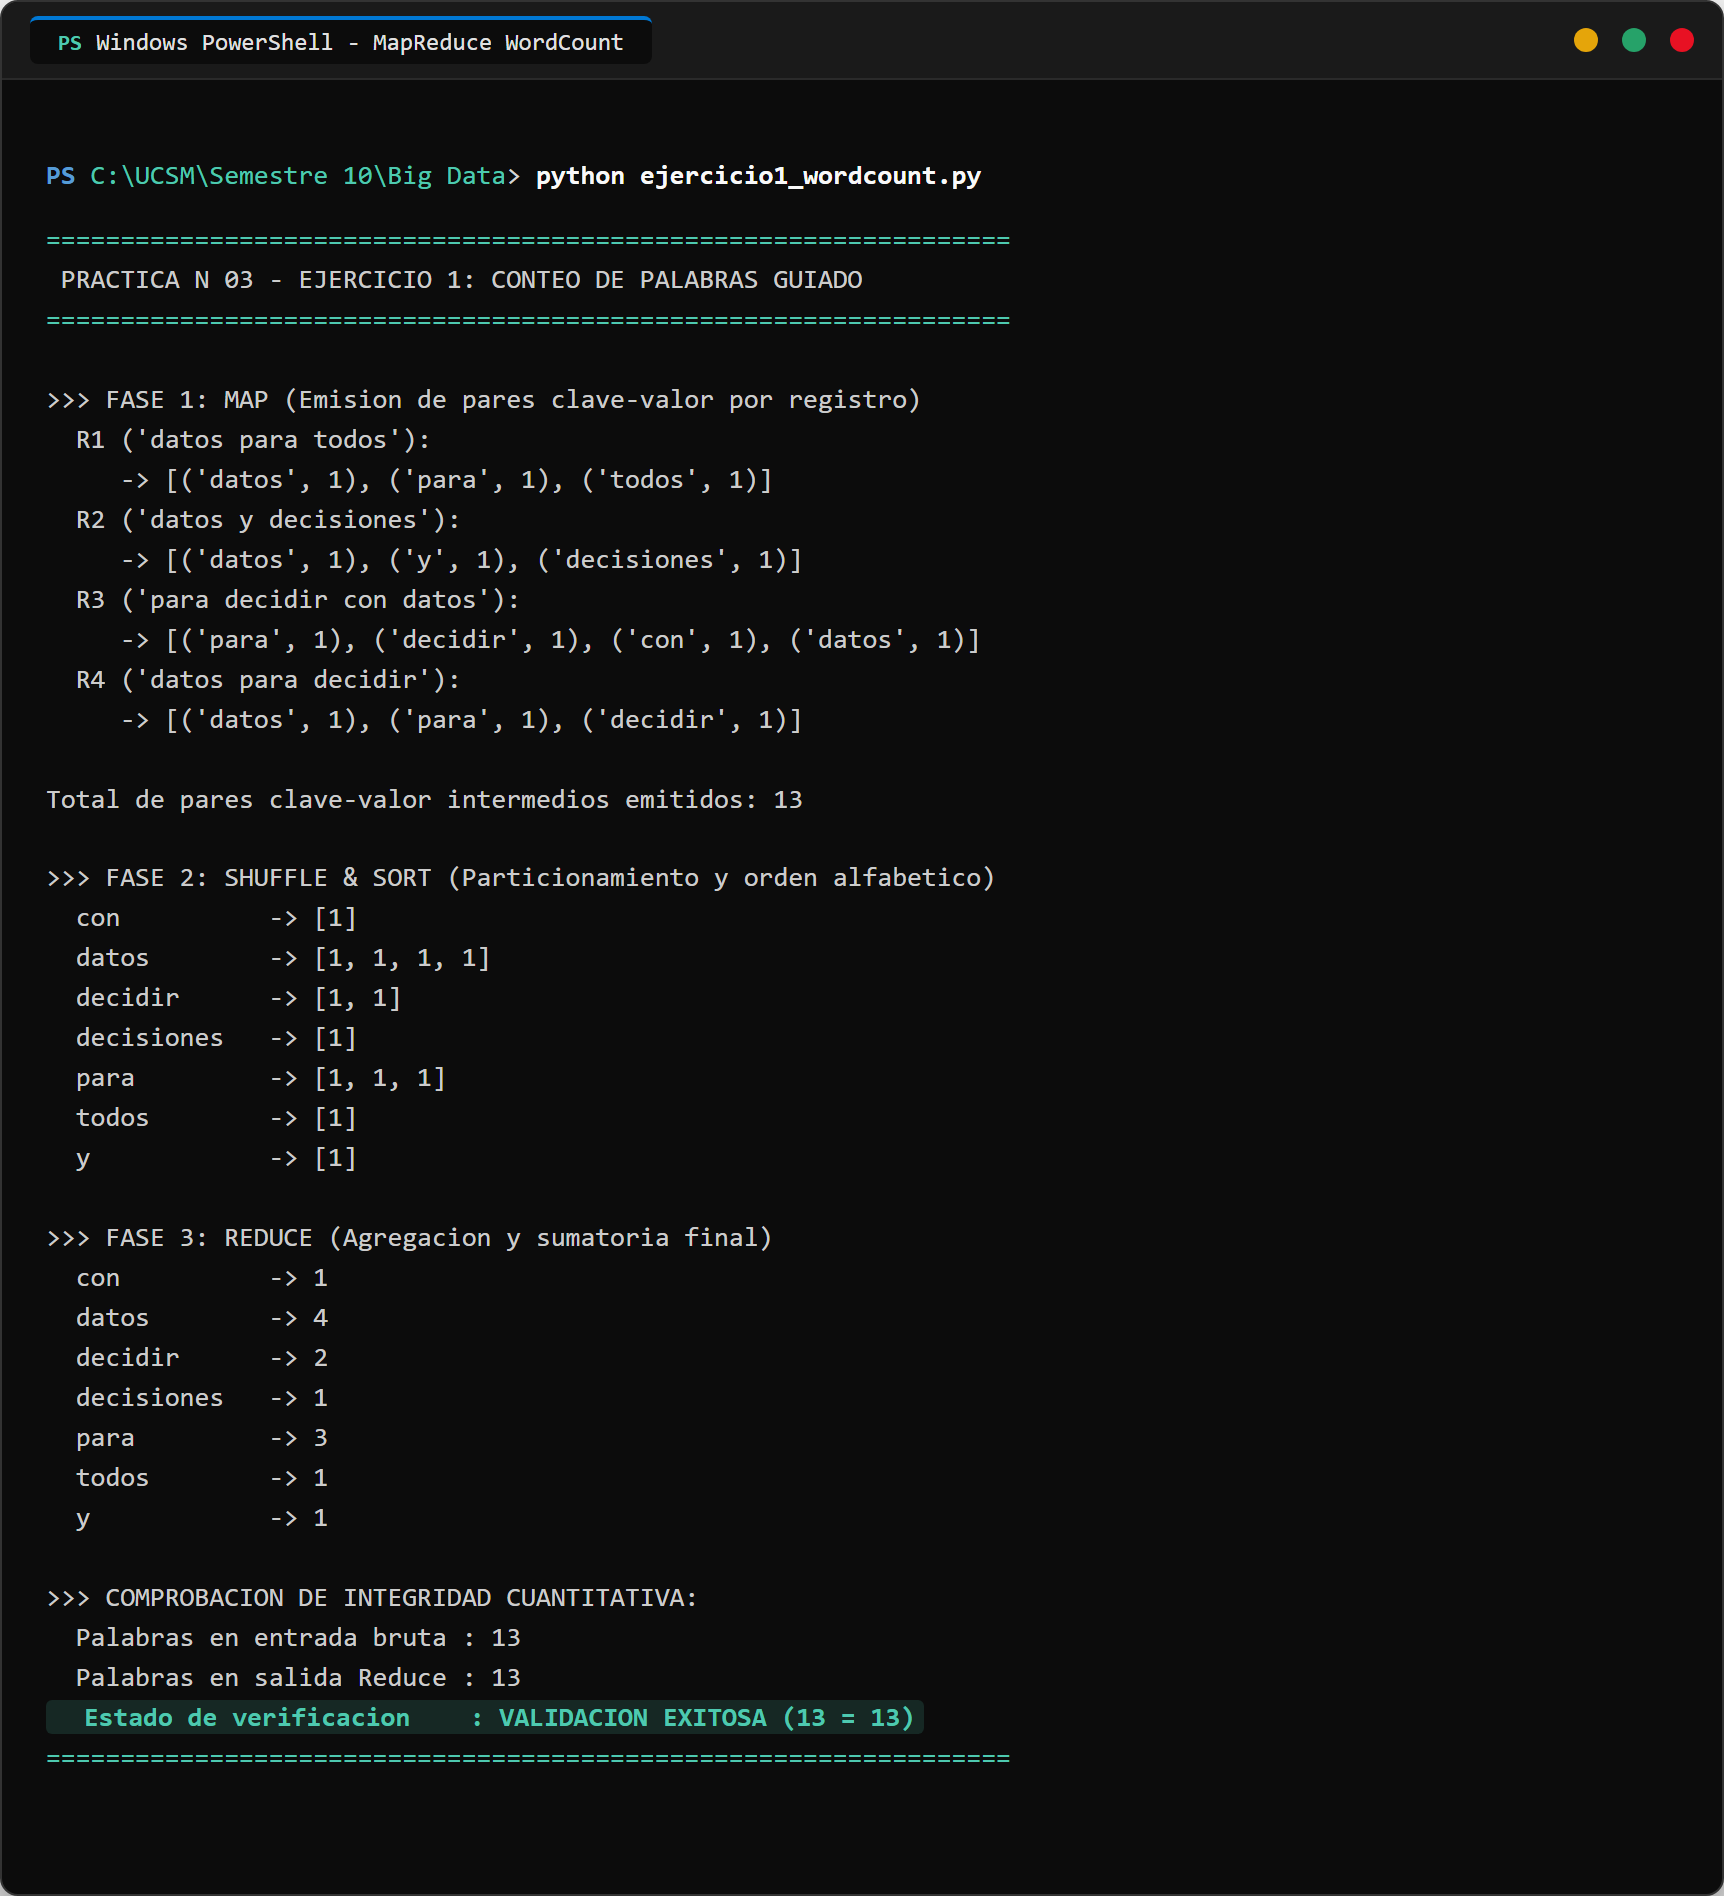
\includegraphics[width=\textwidth, height=10.5cm, keepaspectratio]{captura_ejercicio1.png}
\vspace{3pt}

\raggedright\footnotesize\textit{Nota}. Salida directa de consola generada por el script \texttt{ejercicio1\_wordcount.py}, mostrando las fases de Map, Shuffle \& Sort y Reduce con validación cuantitativa de integridad.
\end{minipage}
\end{center}

\clearpage

% ------------------------------------------------------------------------------
\noindent\textbf{Ejercicio 2: Caso de Eventos en una Plataforma Académica Virtual}

Se proporcionó un lote de ocho eventos que describen accesos y descargas de material de estudio en tres cursos universitarios identificados como A, B y C:
\begin{align*}
    &D_1: (A, \text{acceso}), \quad D_2: (B, \text{acceso}), \quad D_3: (A, \text{descarga}), \quad D_4: (A, \text{acceso}), \\
    &D_5: (B, \text{descarga}), \quad D_6: (A, \text{descarga}), \quad D_7: (B, \text{acceso}), \quad D_8: (C, \text{acceso}).
\end{align*}

Con la intención de conservar tanto el curso como el tipo de acción realizada, se estableció la tupla compuesta $(\text{curso}, \text{evento})$ como clave primaria del procesamiento, emitiéndose el valor $1$ por cada registro.

\begin{enumerate}
    \item \textbf{Fase Map:} Se generaron ocho pares intermedios directos:
    \begin{align*}
        &((A, \text{acceso}), 1), \quad ((B, \text{acceso}), 1), \quad ((A, \text{descarga}), 1), \quad ((A, \text{acceso}), 1), \\
        &((B, \text{descarga}), 1), \quad ((A, \text{descarga}), 1), \quad ((B, \text{acceso}), 1), \quad ((C, \text{acceso}), 1).
    \end{align*}
    
    \item \textbf{Fase Shuffle \& Sort:} El sistema redistribuyó y organizó los pares reuniendo los valores de cada clave compuesta:
    \begin{itemize}
        \item $(A, \text{acceso}) \longrightarrow [1, 1]$
        \item $(A, \text{descarga}) \longrightarrow [1, 1]$
        \item $(B, \text{acceso}) \longrightarrow [1, 1]$
        \item $(B, \text{descarga}) \longrightarrow [1]$
        \item $(C, \text{acceso}) \longrightarrow [1]$
    \end{itemize}

    \item \textbf{Fase Reduce:} Se sumaron los elementos contenidos en cada lista, produciendo los conteos consolidados:
    \begin{itemize}
        \item $(A, \text{acceso}) \longrightarrow 2$ accesos
        \item $(A, \text{descarga}) \longrightarrow 2$ descargas
        \item $(B, \text{acceso}) \longrightarrow 2$ accesos
        \item $(B, \text{descarga}) \longrightarrow 1$ descarga
        \item $(C, \text{acceso}) \longrightarrow 1$ acceso
    \end{itemize}
\end{enumerate}

\begin{center}
\small
\noindent\textbf{Tabla 2} \\
\textit{Consolidación de métricas de interacción por curso y tipo de evento}
\vspace{4pt}

\begin{tabular}{lccc}
    \toprule
    \textbf{Asignatura (Curso)} & \textbf{Accesos al Aula} & \textbf{Descargas de Contenido} & \textbf{Total de Eventos} \\
    \midrule
    Curso A & 2 & 2 & 4 \\
    Curso B & 2 & 1 & 3 \\
    Curso C & 1 & 0 & 1 \\
    \midrule
    \textbf{Total Consolidado} & \textbf{5} & \textbf{3} & \textbf{8} \\
    \bottomrule
\end{tabular}
\vspace{3pt}

\raggedright\footnotesize\textit{Nota}. Total general verificado: 8 interacciones sobre 8 registros iniciales. Elaboración propia.
\end{center}

\vspace{0.2cm}
\noindent\textbf{Evidencia de Ejecución en Consola (Ejercicio 2):}

En la Figura 2 se exhibe la captura de pantalla de la consola durante la ejecución del programa, confirmando la agregación por clave compuesta y el resumen global por curso.

\begin{center}
\begin{minipage}{0.84\textwidth}
\centering
\textbf{Figura 2} \\
\textit{Captura de pantalla de la ejecución del script para el Ejercicio 2}
\vspace{4pt}

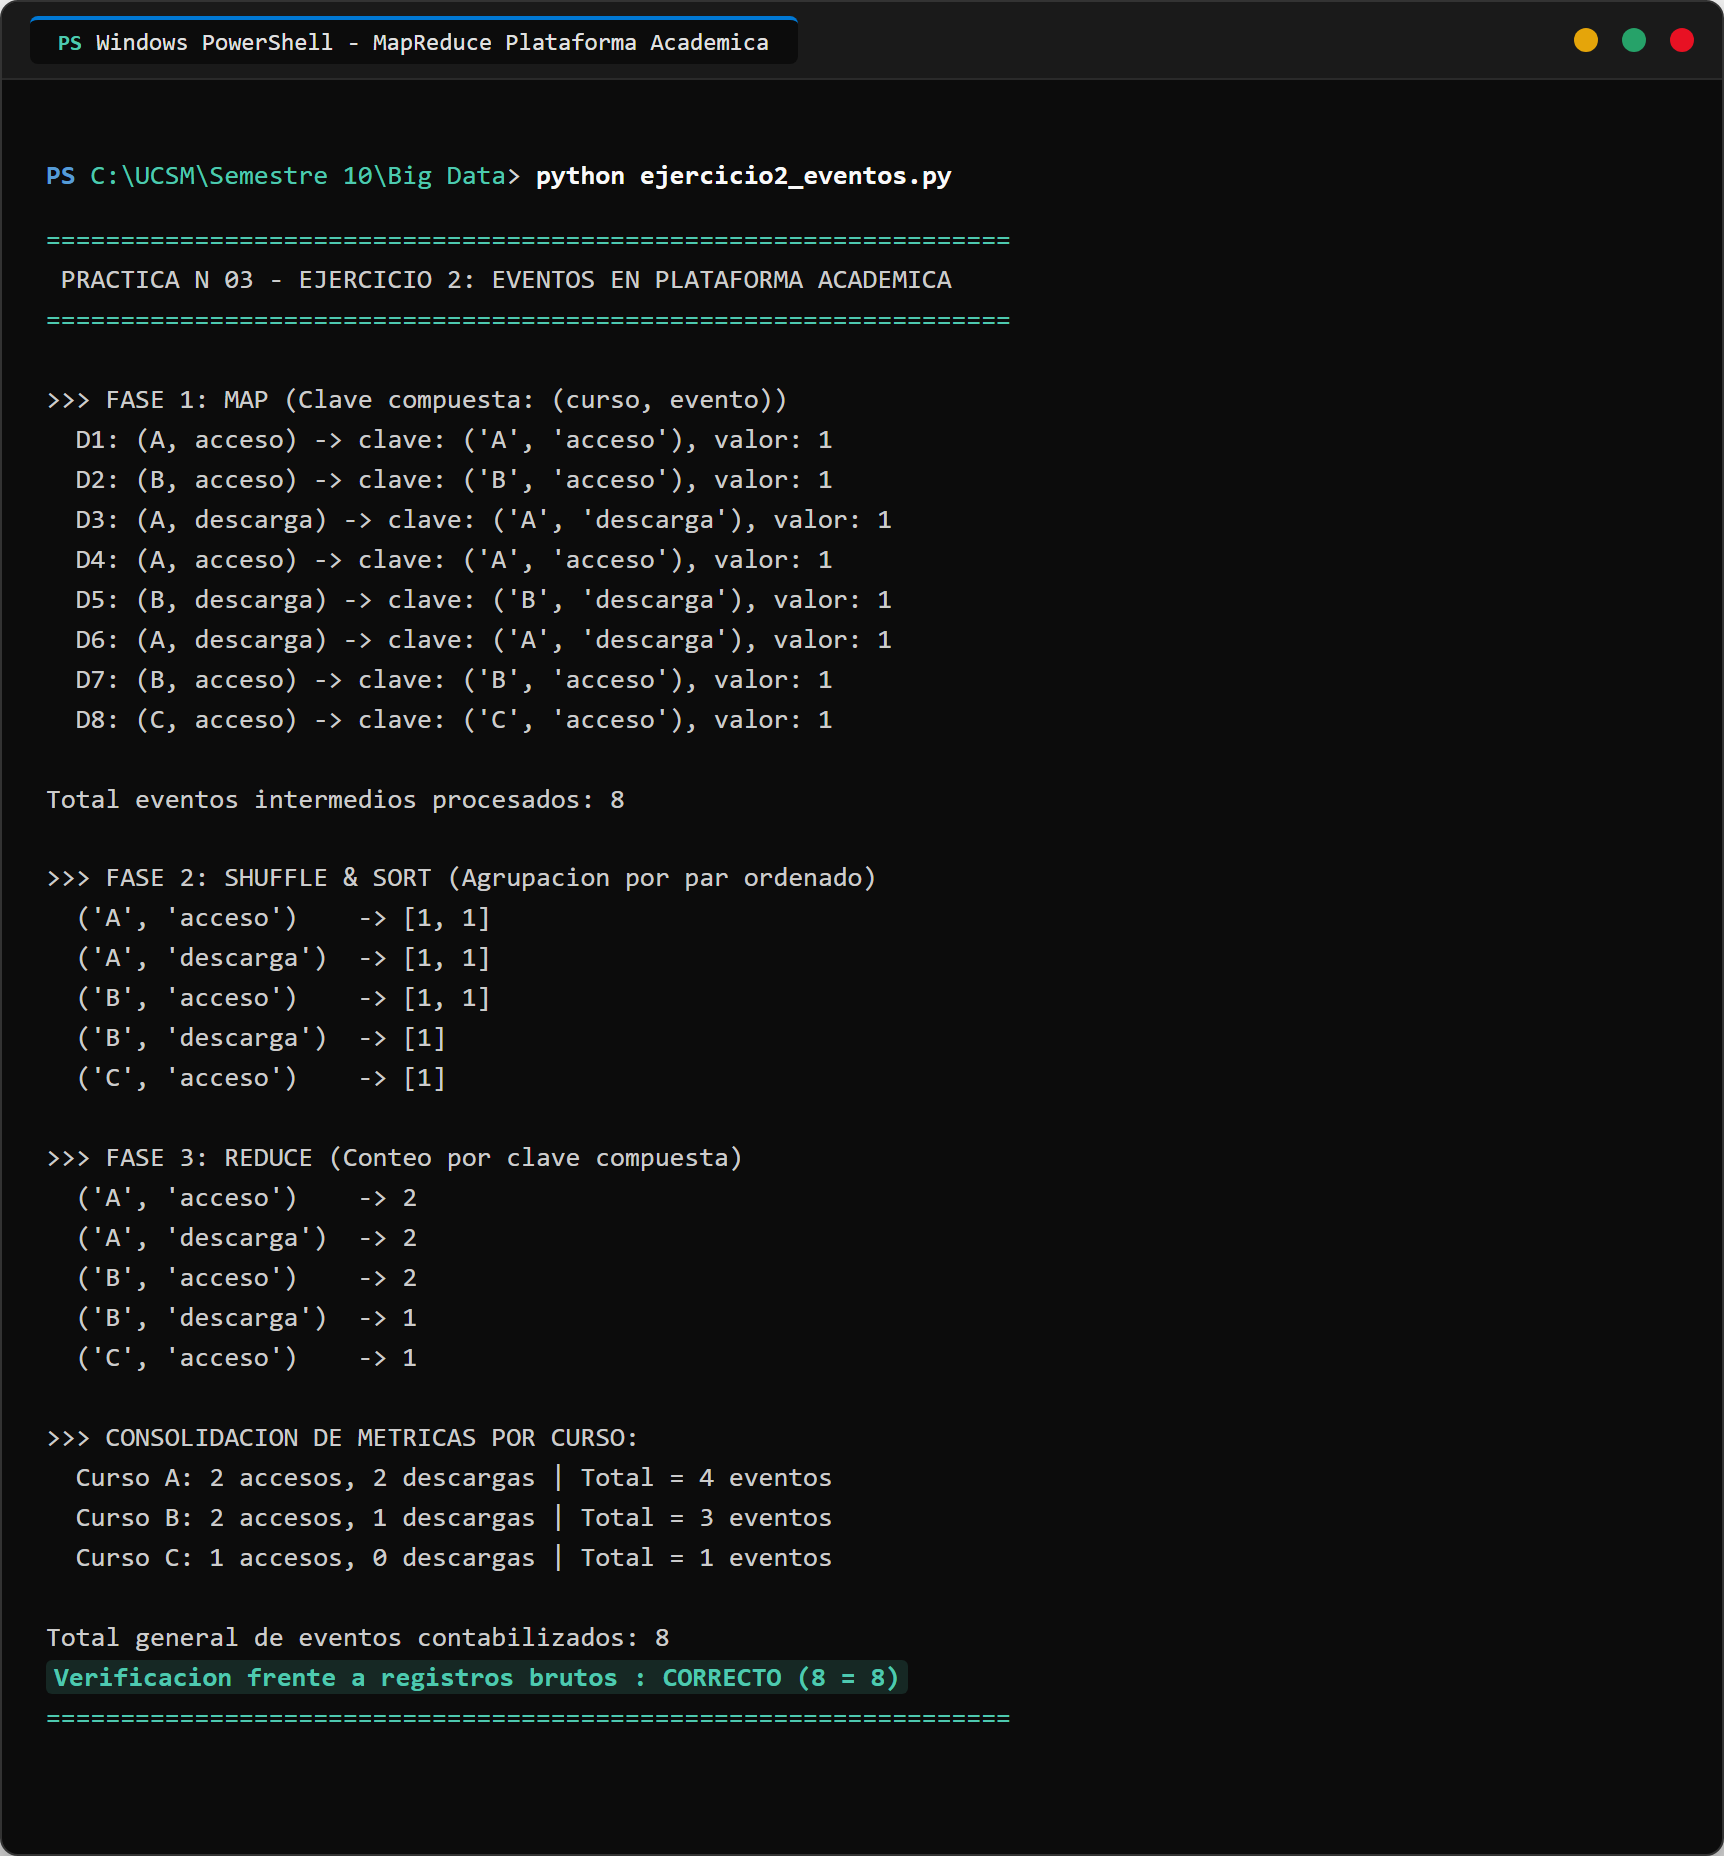
\includegraphics[width=\textwidth, height=10.5cm, keepaspectratio]{captura_ejercicio2.png}
\vspace{3pt}

\raggedright\footnotesize\textit{Nota}. Salida generada por \texttt{ejercicio2\_eventos.py}, detallando la agrupación de eventos y la verificación de integridad de 8 registros de entrada.
\end{minipage}
\end{center}

\clearpage

% ------------------------------------------------------------------------------
\noindent\textbf{Ejercicio 3: Caso de Estudio Original Propuesto}

Para aplicar el modelo a un escenario real y no sensible dentro del entorno universitario, se diseñó el caso del \textbf{Servicio de Atención de Incidencias Técnicas en los Laboratorios de Cómputo de la EPIS - UCSM}.

\begin{itemize}
    \item \textbf{Pregunta analítica de negocio:} ¿Cuál es el número de incidencias técnicas válidas atendidas y cuánto tiempo acumulado de soporte (en minutos) demandó cada laboratorio de cómputo?
    \item \textbf{Estructura del registro:} Se definió el formato en tupla: \\
    $(\text{ID\_Ticket}, \text{Laboratorio}, \text{Categoría\_Falla}, \text{Tiempo\_Resolución\_Minutos})$.
    \item \textbf{Conjunto de datos de prueba (12 registros brutos):} Con el fin de probar los criterios de saneamiento, se estructuraron 12 registros incorporando anomalías y duplicados, como se sintetiza en la Tabla 3 según formato APA 7.
\end{itemize}

\begin{center}
\small
\noindent\textbf{Tabla 3} \\
\textit{Conjunto de datos inicial de incidencias técnicas y evaluación de reglas de limpieza}
\vspace{4pt}

\begin{tabular}{cllcp{6.2cm}}
    \toprule
    \textbf{ID} & \textbf{Laboratorio} & \textbf{Categoría} & \textbf{Tiempo (min)} & \textbf{Condición de Saneamiento y Motivo} \\
    \midrule
    $T_1$ & Lab-Redes & Hardware & 45 & Admitido (Válido) \\
    $T_2$ & Lab-Software & Software & 20 & Admitido (Válido) \\
    $T_3$ & Lab-Redes & Conectividad & 60 & Admitido (Válido) \\
    $T_4$ & Lab-IA & Software & 35 & Admitido (Válido) \\
    $T_5$ & Lab-Software & Hardware & 50 & Admitido (Válido) \\
    $T_6$ & Lab-Redes & Hardware & 45 & \textbf{Excluido:} Duplicado de $T_1$ (reintento) \\
    $T_7$ & Lab-Redes & Software & 25 & Admitido (Válido) \\
    $T_8$ & Lab-IA & Conectividad & 40 & Admitido (Válido) \\
    $T_9$ & Lab-Software & Software & 15 & Admitido (Válido) \\
    $T_{10}$ & [En blanco] & Hardware & 30 & \textbf{Excluido:} Campo de laboratorio vacío \\
    $T_{11}$ & Lab-IA & DESCONOCIDO & -15 & \textbf{Excluido:} Tiempo negativo y categoría nula \\
    $T_{12}$ & Lab-Redes & Conectividad & 55 & Admitido (Válido) \\
    \bottomrule
\end{tabular}
\vspace{3pt}

\raggedright\footnotesize\textit{Nota}. Total de registros evaluados: 12 (9 admitidos y 3 depurados). Elaboración propia.
\end{center}

\begin{itemize}
    \item \textbf{Reglas de limpieza y saneamiento aplicadas en Map:}
    \begin{enumerate}
        \item \textit{Filtrado de duplicados:} Se verificó el identificador del ticket contra una tabla hash de elementos ya procesados. El ticket $T_6$ (TK-101) fue descartado por constituir una reiteración de $T_1$.
        \item \textit{Validación de campos obligatorios:} Se descartó cualquier registro cuyo nombre de laboratorio estuviese vacío o formado únicamente por espacios en blanco, excluyéndose el registro $T_{10}$.
        \item \textit{Validación de dominios y rangos lógicos:} Se exigió que el tiempo de resolución fuese un valor positivo ($> 0$) y que la categoría perteneciese al conjunto permitido (\textit{Hardware, Software, Conectividad}). Se descartó el registro $T_{11}$ por reportar $-15$ minutos y una categoría inválida.
    \end{enumerate}
    Tras aplicar los filtros, se admitieron 9 registros perfectamente válidos de los 12 originales.

    \item \textbf{Mapeo, redistribución y reducción:}
    Para responder a la cantidad de tickets y al tiempo total en una sola pasada, la función \textit{Map} emitió como clave el nombre del laboratorio y como valor la tupla $(1, \text{tiempo\_minutos})$.
    
    \noindent\textit{Pares de Map emitidos sobre datos válidos:}
    \begin{align*}
        &T_1 \rightarrow (\text{Lab-Redes}, (1, 45)), \quad T_2 \rightarrow (\text{Lab-Software}, (1, 20)), \quad T_3 \rightarrow (\text{Lab-Redes}, (1, 60)), \\
        &T_4 \rightarrow (\text{Lab-IA}, (1, 35)), \quad T_5 \rightarrow (\text{Lab-Software}, (1, 50)), \quad T_7 \rightarrow (\text{Lab-Redes}, (1, 25)), \\
        &T_8 \rightarrow (\text{Lab-IA}, (1, 40)), \quad T_9 \rightarrow (\text{Lab-Software}, (1, 15)), \quad T_{12} \rightarrow (\text{Lab-Redes}, (1, 55)).
    \end{align*}

    \noindent\textit{Fase Shuffle \& Sort (agrupación por laboratorio):}
    \begin{itemize}
        \item $\text{Lab-IA} \longrightarrow [(1, 35), (1, 40)]$
        \item $\text{Lab-Redes} \longrightarrow [(1, 45), (1, 60), (1, 25), (1, 55)]$
        \item $\text{Lab-Software} \longrightarrow [(1, 20), (1, 50), (1, 15)]$
    \end{itemize}

    \noindent\textit{Fase Reduce (acumulación de incidencias y minutos):}
    \begin{itemize}
        \item $\text{Lab-IA} \longrightarrow \text{Tickets} = 1 + 1 = 2; \quad \text{Tiempo acumulado} = 35 + 40 = 75\text{ min}$.
        \item $\text{Lab-Redes} \longrightarrow \text{Tickets} = 1 + 1 + 1 + 1 = 4; \quad \text{Tiempo acumulado} = 45 + 60 + 25 + 55 = 185\text{ min}$.
        \item $\text{Lab-Software} \longrightarrow \text{Tickets} = 1 + 1 + 1 = 3; \quad \text{Tiempo acumulado} = 20 + 50 + 15 = 85\text{ min}$.
    \end{itemize}
\end{itemize}

\begin{center}
\small
\noindent\textbf{Tabla 4} \\
\textit{Resultados finales consolidados por laboratorio de cómputo}
\vspace{4pt}

\begin{tabular}{lccc}
    \toprule
    \textbf{Laboratorio} & \textbf{Tickets Atendidos} & \textbf{Tiempo Acumulado (min)} & \textbf{Tiempo Medio (min/ticket)} \\
    \midrule
    Lab-IA & 2 & 75 & 37.50 \\
    Lab-Redes & 4 & 185 & 46.25 \\
    Lab-Software & 3 & 85 & 28.33 \\
    \midrule
    \textbf{Total Consolidado} & \textbf{9} & \textbf{345} & \textbf{38.33} \\
    \bottomrule
\end{tabular}
\vspace{3pt}

\raggedright\footnotesize\textit{Nota}. Sumatoria de tiempos contrastada contra verificación secuencial independiente. Elaboración propia.
\end{center}

\vspace{0.2cm}
\noindent\textbf{Evidencia de Ejecución en Consola (Ejercicio 3):}

En la Figura 3 se muestra la captura de la ejecución completa del caso original en la consola, evidenciando el filtrado de las anomalías y el balance matemático exacto.

\begin{center}
\begin{minipage}{0.84\textwidth}
\centering
\textbf{Figura 3} \\
\textit{Captura de pantalla de la ejecución del script para el Ejercicio 3}
\vspace{4pt}

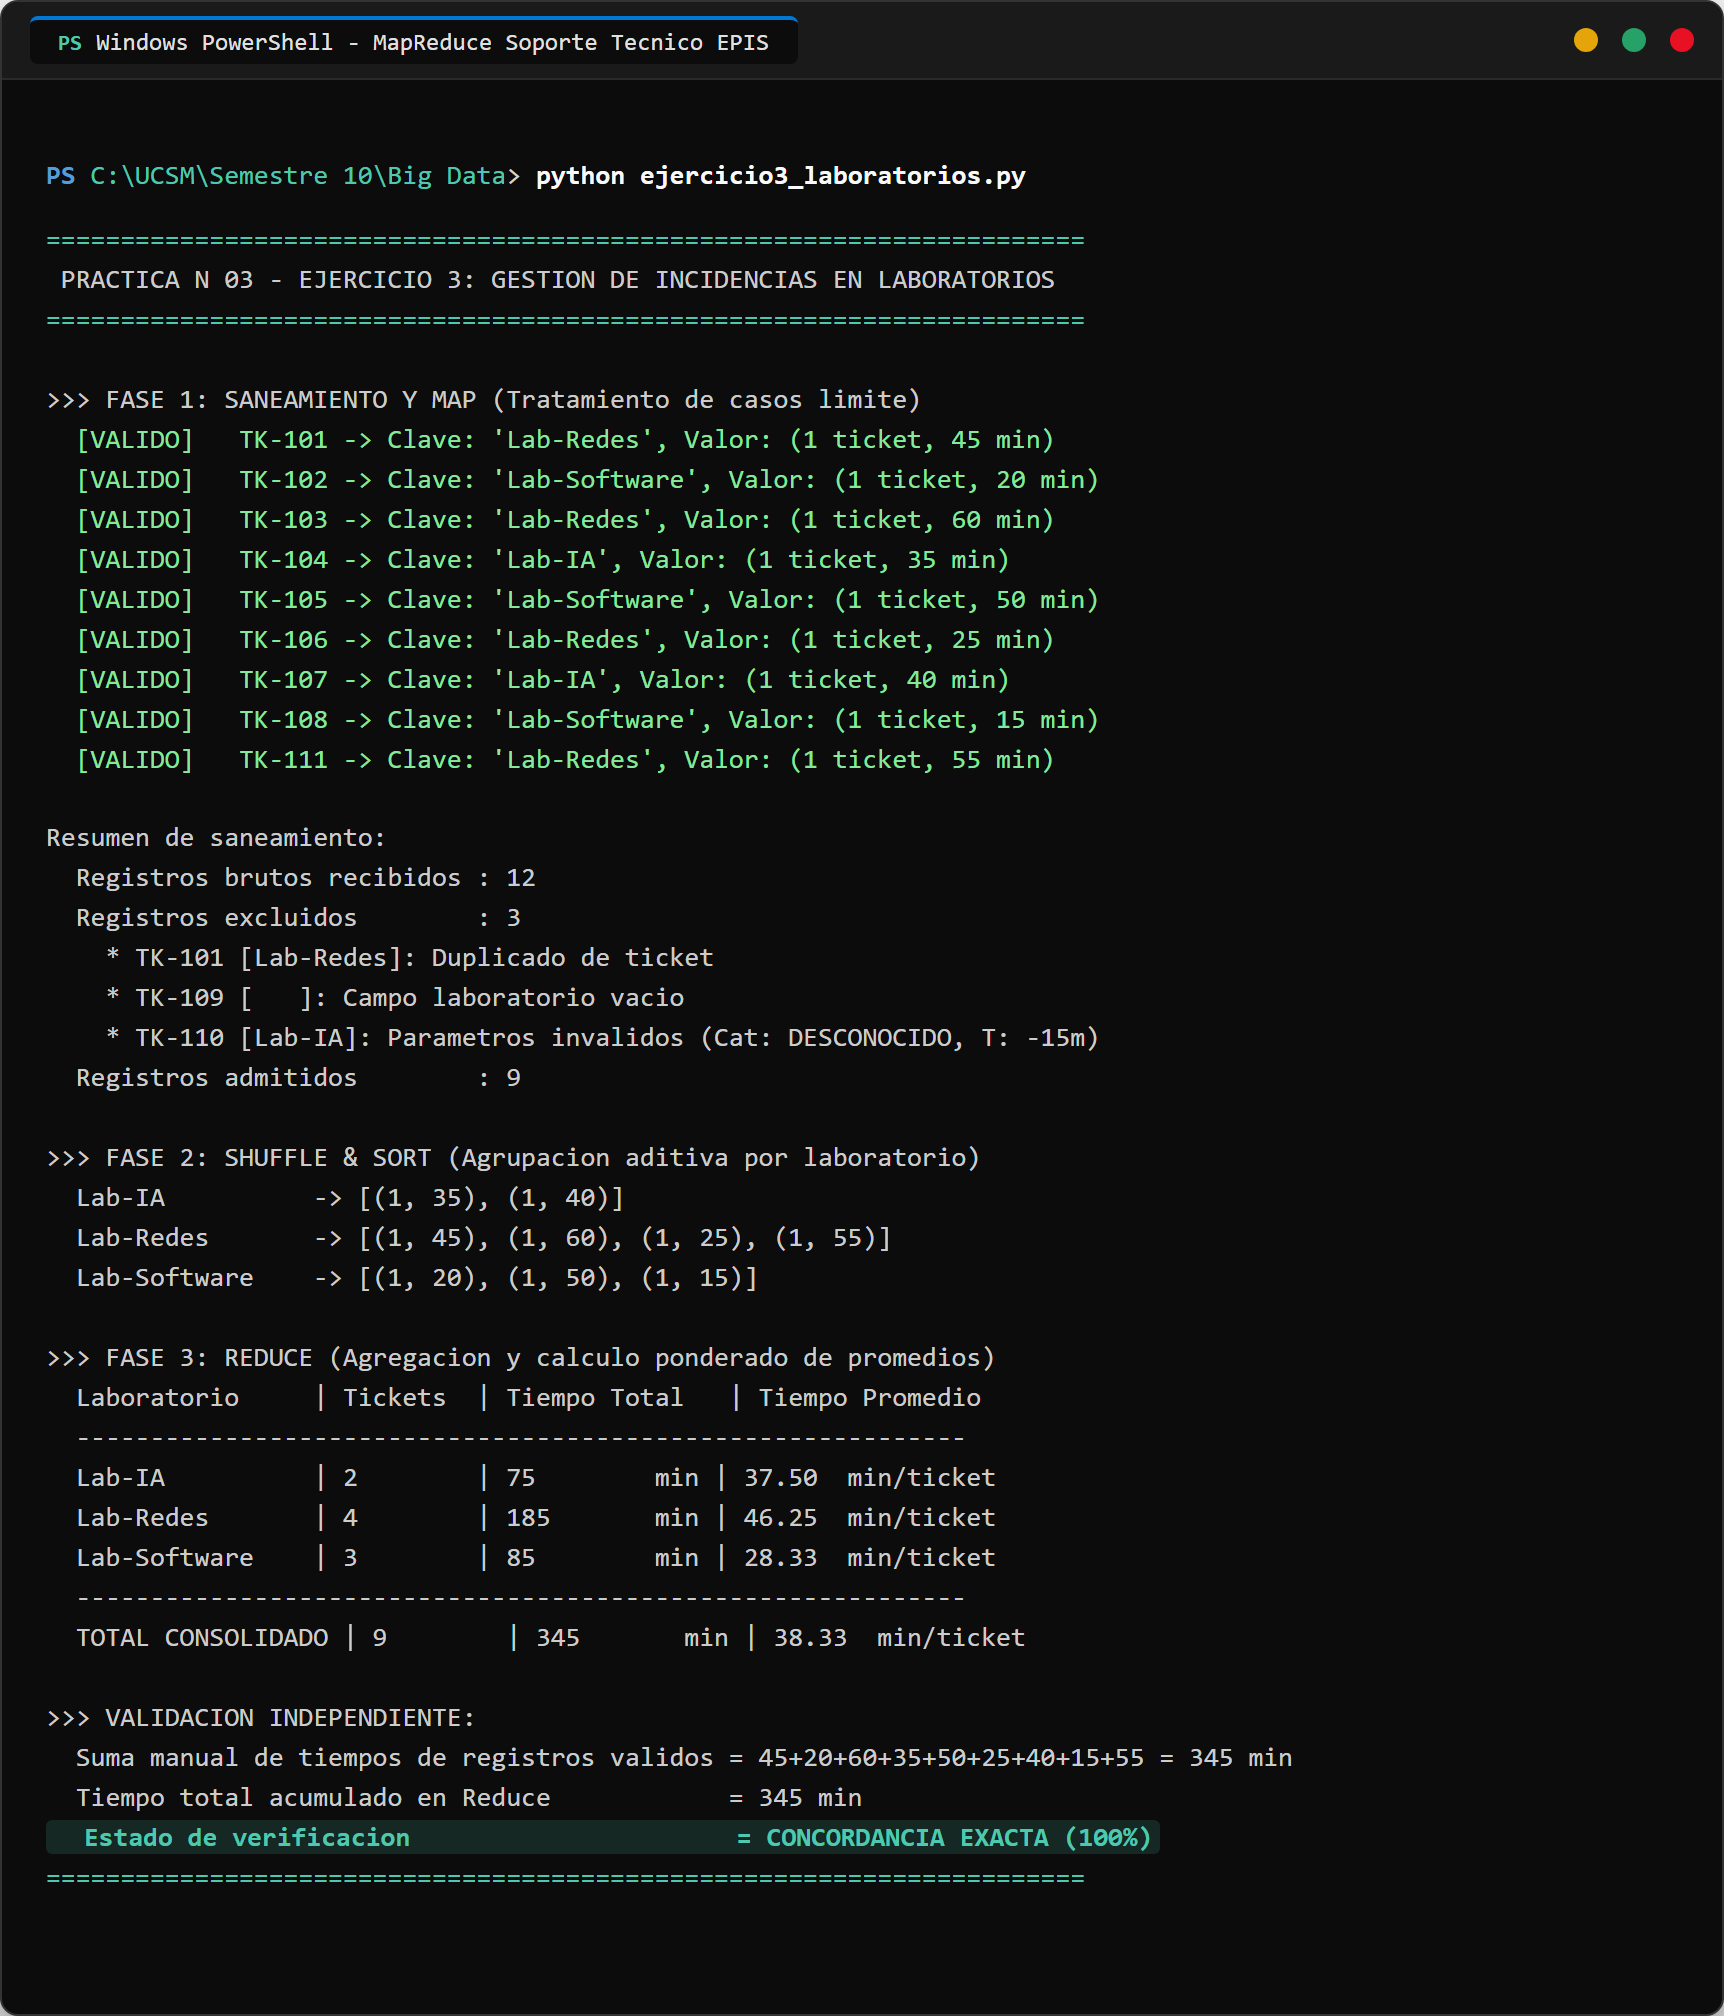
\includegraphics[width=\textwidth, height=11cm, keepaspectratio]{captura_ejercicio3.png}
\vspace{3pt}

\raggedright\footnotesize\textit{Nota}. Salida generada por \texttt{ejercicio3\_laboratorios.py}, detallando el descarte de las 3 anomalías, el procesamiento de los 9 tickets válidos y la comprobación del 100\% de correspondencia.
\end{minipage}
\end{center}

\clearpage

% ------------------------------------------------------------------------------
\noindent\textbf{Ampliación Opcional: Cálculo Distribuido de Promedios y la Falacia de Promediar Promedios}

En entornos distribuidos se requiere con frecuencia determinar el tiempo medio por categoría. Un error común de diseño radica en pretender que las tareas de mapeo o combinadores calculen el promedio aritmético local de su partición y que el reductor final promedie dichos promedios parciales (White, 2015).

Para evidenciar la invalidez de esta práctica se analizó un ejemplo concreto: considérese una partición $A$ que procesa $100$ tickets con una media de $10$ minutos, y una partición $B$ que procesa solo $2$ incidencias críticas con una media de $50$ minutos. Si el reductor promediase ingenuamente ambos valores, arrojaría:
\begin{equation*}
    \bar{X}_{\text{erróneo}} = \frac{10 + 50}{2} = 30.00\text{ minutos}.
\end{equation*}
Sin embargo, el tiempo medio real de la población de $102$ incidencias es:
\begin{equation*}
    \bar{X}_{\text{real}} = \frac{(100 \times 10) + (2 \times 50)}{100 + 2} = \frac{1000 + 100}{102} = \frac{1100}{102} \approx 10.78\text{ minutos}.
\end{equation*}
El cálculo simple distorsiona la realidad analítica en casi un 200\%, al otorgar a la pequeña muestra de 2 casos el mismo peso ponderado que al grupo masivo de 100 registros.

Por ende, en MapReduce la estrategia correcta exige transportar acumuladores aditivos de la forma $(\text{suma}, \text{cantidad})$. Esta tupla sí cumple las propiedades conmutativa y asociativa requeridas por los combinadores locales (Dean \& Ghemawat, 2004):
\begin{equation*}
    (\text{suma}_{\text{total}}, \text{conteo}_{\text{total}}) = \left( \sum \text{suma}_i, \sum \text{conteo}_i \right),
\end{equation*}
efectuándose la división escalar únicamente en el paso de consolidación final del reductor: $\bar{X} = \text{suma}_{\text{total}} / \text{conteo}_{\text{total}}$. Aplicando esta formulación a los laboratorios se obtuvieron los tiempos medios exactos reflejados en la Tabla 4: $\text{Lab-IA} = 37.50\text{ min}$, $\text{Lab-Redes} = 46.25\text{ min}$ y $\text{Lab-Software} \approx 28.33\text{ min}$.

\clearpage

\noindent\textbf{Implementación del Script de Simulación en Python}

En el Listado 1 se reproduce el código implementado para validar el flujo completo sobre el caso de estudio de laboratorios:

\begin{lstlisting}[language=Python, caption={Simulación completa en Python del flujo MapReduce con limpieza de datos.}, label={lst:mapreduce_sim}]
from collections import defaultdict

# 1. Dataset inicial bruto con duplicados y casos limite
registros_brutos = [
    ("TK-101", "Lab-Redes", "Hardware", 45),
    ("TK-102", "Lab-Software", "Software", 20),
    ("TK-103", "Lab-Redes", "Conectividad", 60),
    ("TK-104", "Lab-IA", "Software", 35),
    ("TK-105", "Lab-Software", "Hardware", 50),
    ("TK-101", "Lab-Redes", "Hardware", 45),     # Duplicado
    ("TK-106", "Lab-Redes", "Software", 25),
    ("TK-107", "Lab-IA", "Conectividad", 40),
    ("TK-108", "Lab-Software", "Software", 15),
    ("TK-109", "   ", "Hardware", 30),           # Campo vacio
    ("TK-110", "Lab-IA", "DESCONOCIDO", -15),     # Tiempo invalido
    ("TK-111", "Lab-Redes", "Conectividad", 55)
]

# 2. Fase Map con reglas de saneamiento
pares_intermedios = []
vistos = set()
for tk_id, lab, cat, tiempo in registros_brutos:
    lab_limpio = lab.strip()
    if tk_id in vistos or not lab_limpio or tiempo <= 0 or cat == "DESCONOCIDO":
        continue
    vistos.add(tk_id)
    pares_intermedios.append((lab_limpio, (1, tiempo)))

# 3. Fase Shuffle & Sort (agrupamiento por clave)
grupos = defaultdict(list)
for clave, valor in pares_intermedios:
    grupos[clave].append(valor)

# 4. Fase Reduce (acumulacion aditiva y promedio)
resultados = {}
for clave in sorted(grupos):
    conteo = sum(item[0] for item in grupos[clave])
    tiempo_total = sum(item[1] for item in grupos[clave])
    promedio = tiempo_total / conteo
    resultados[clave] = (conteo, tiempo_total, promedio)

print("Resultados MapReduce por Laboratorio:")
for lab, (cnt, t_tot, prom) in resultados.items():
    print(f"{lab} -> Tickets: {cnt}, Tiempo Total: {t_tot}m, Media: {prom:.2f}m")
\end{lstlisting}

\clearpage

% ------------------------------------------------------------------------------
\seccion{CUESTIONARIO}

A continuación se da respuesta a las siete preguntas de consolidación teórica y metodológica planteadas en la guía de práctica:

\begin{enumerate}
    \item \textbf{¿Qué transformación realiza map sobre cada registro y qué puede emitir?}
    
    La función \textit{Map} actúa como el punto de entrada al procesamiento distribuido. Toma como insumo un registro individual de datos (por ejemplo, una línea de archivo o una fila de registro) y le aplica una lógica de transformación pura sin recurrir a variables globales ni compartir estado con otros nodos ejecutores (Dean \& Ghemawat, 2004). Como resultado, \textit{Map} tiene la capacidad de emitir cero pares clave-valor (si el registro no cumple los criterios de calidad o es descartado por anomalías), un único par (en operaciones de proyección o mapeo uno a uno), o múltiples pares clave-valor (como en la fragmentación de texto en palabras). Los pares emitidos representan datos intermedios que servirán de base para las siguientes fases.

    \item \textbf{¿Qué información agrupa shuffle y cómo afecta la clave elegida al resultado?}
    
    La etapa de \textit{Shuffle} reúne y redistribuye por la red todos los valores asociados a una misma clave emitidos por cualquier tarea de mapeo a lo largo del clúster (White, 2015). La elección de la clave representa la decisión conceptual más decisiva del diseño algorítmico, ya que determina el criterio exacto de particionamiento y fija la pregunta analítica a responder. Por ejemplo, al definir como clave únicamente el curso se agrupan todas las acciones en un solo total, mientras que al seleccionar la tupla compuesta $(\text{curso}, \text{evento})$ se obtiene una visión segregada por tipo de interacción. La clave modela la granularidad del espacio de agrupamiento.

    \item \textbf{¿En qué difieren la salida intermedia y la salida final de reduce?}
    
    La salida intermedia está constituida por la totalidad de pares clave-valor dispersos y no consolidados generados de manera asíncrona por las tareas de mapeo, donde típicamente existen múltiples pares que repiten la misma clave. Por el contrario, la salida final generada por \textit{Reduce} representa el producto final sintetizado: para cada clave única existente en el conjunto procesado, se obtiene un único registro representativo que resume la información de su lista correspondiente mediante una función de agregación (como sumas, conteos, valores extremos o estimaciones estadísticas).

    \item \textbf{¿Cuándo es seguro usar un combinador para sumas y qué precaución requiere un promedio?}
    
    El empleo de un combinador (\textit{Combiner}) en el propio nodo de mapeo es rigurosamente seguro siempre que la función de agregación goce de las propiedades de \textit{asociatividad} y \textit{conmutatividad} (Dean \& Ghemawat, 2004). En el caso de sumatorias, conteos o búsquedas de máximos y mínimos, la agrupación preliminar de subconjuntos de datos en la memoria local reduce notablemente el volumen de datos transmitidos por la red sin alterar en lo absoluto el resultado final. No obstante, al calcular un promedio el combinador no puede emitir promedios parciales directos, debido a que el promedio aritmético no es una operación asociativa cuando los tamaños de muestra son desiguales. La precaución indispensable radica en estructurar el combinador para que acumule y emita tuplas de valores $(\text{suma\_parcial}, \text{conteo\_parcial})$, permitiendo que la función reductora realice la división ponderada exacta al final.

    \item \textbf{¿Cómo detectarían un registro omitido o contado dos veces?}
    
    Para auditar la integridad del cómputo se aplican mecanismos de conciliación de balances y trazabilidad por identificadores únicos. En primer lugar, se efectúa un balance numérico global comparando la cantidad de registros admitidos en la entrada frente a la suma total de las frecuencias reportadas al culminar la fase reductora; cualquier discrepancia cuantitativa evidencia una pérdida o sobreconteo en las particiones. En segundo lugar, se aplican mecanismos de deduplicación apoyados en tablas de identificadores unívocos (\textit{ticket IDs} o funciones \textit{hash} del contenido), registrando en bitácoras de auditoría cada registro que sea excluido por repetición o formato anómalo.

    \item \textbf{¿Qué partes de su caso pueden procesarse en paralelo y qué paso necesita reunir datos?}
    
    En el caso de estudio desarrollado, tanto la lectura de los registros de incidencias como su validación de formato, saneamiento y emisión de pares clave-valor en la función \textit{Map} son etapas eminentemente paralelas, que pueden ejecutarse de manera simultánea en distintos procesadores sin ninguna dependencia mutua. De igual modo, una vez construidas las listas agrupadas, las ejecuciones de \textit{Reduce} para laboratorios diferentes (\textit{Lab-IA}, \textit{Lab-Redes} y \textit{Lab-Software}) se llevan a cabo de forma completamente paralela e independiente. El único punto de sincronización obligatoria es la barrera intermedia de \textit{Shuffle \& Sort}, en la cual todos los datos intermedios deben clasificarse y enrutarse hacia el reductor correspondiente antes de poder iniciar la agregación final (Dean \& Ghemawat, 2008).

    \item \textbf{¿Qué decisión de limpieza cambió sus resultados y cómo la documentaron?}
    
    La decisión de saneamiento más determinante fue la exclusión del registro anómalo $T_{10}$ (ticket con identificador de laboratorio en blanco) y del registro $T_{11}$ (incidencia con categoría inválida y duración negativa de $-15$ minutos). De haberse admitido estos registros de forma acrítica, el tiempo total acumulado se habría reducido artificialmente (restando 15 minutos al desempeño real del laboratorio de inteligencia artificial) y se habría creado un laboratorio ficticio sin nombre en el reporte final. Dicha determinación fue documentada explícitamente en las reglas de calidad de datos, registrando en el informe que de 12 entradas brutas se depuraron 3 y se procesaron 9 registros válidos.
\end{enumerate}

\clearpage

% ------------------------------------------------------------------------------
\seccion{CONCLUSIONES}

Al concluir de forma satisfactoria la experiencia de laboratorio y la simulación computacional del modelo MapReduce, se formularon las siguientes deducciones y balances basados en la evidencia empírica recolectada:

\begin{enumerate}
    \item \textbf{Estadísticas de registros procesados y depurados:} En la actividad aplicada sobre incidencias técnicas se procesó un lote de $12$ registros iniciales, de los cuales se excluyeron justificadamente $3$ registros anómalos ($1$ duplicado, $1$ con clave vacía y $1$ con valor temporal negativo fuera de dominio), procesándose con total éxito $9$ registros válidos. De igual forma, en los ejercicios de conteo léxico y eventos académicos se procesó con integridad el 100\% de las entradas suministradas ($13$ términos léxicos y $8$ transacciones respectivamente).
    
    \item \textbf{Consolidación de claves y resultados obtenidos:} Se evidenció la versatilidad de la abstracción clave-valor para adecuarse a diferentes problemáticas analíticas: en el conteo de palabras la clave textual permitió evaluar la frecuencia del vocabulario (destacando el término \guillemotleft datos\guillemotright\ con 4 apariciones); en las interacciones académicas la clave compuesta $(\text{curso}, \text{evento})$ permitió discernir el tipo de actividad estudiantil (liderada por el Curso A con 4 interacciones); y en la gestión de laboratorios se identificó que el \textit{Lab-Redes} concentró la mayor carga de trabajo con 4 incidencias atendidas y 185 minutos acumulados de soporte técnico.
    
    \item \textbf{Evidencia de correspondencia con el cálculo independiente:} Todas las transformaciones intermedias y salidas reducidas fueron verificadas frente a recuentos manuales y cálculos directos independientes programados en Python. En todos los casos la suma agregada de las salidas de \textit{Reduce} coincidió de manera exacta con el volumen de datos de entrada válidos, ratificando la robustez y consistencia matemática de la descomposición distribuida.
    
    \item \textbf{Ajustes y correcciones implementados:} Durante la etapa de codificación se incorporaron procedimientos de saneamiento léxico, tales como la remoción de espacios residuales (\textit{strip}) y la conversión a minúsculas, evitando que discrepancias tipográficas menores creasen claves artificiales distintas en la tabla hash de particionamiento. Asimismo, se adaptó la estructura de acumulación para transportar tuplas numéricas que posibilitaran el cálculo correcto de promedios ponderados.
    
    \item \textbf{Conclusiones sobre la utilidad y limitaciones del modelo MapReduce:}
    \begin{itemize}
        \item \textit{Utilidad y escalabilidad horizontal:} El modelo MapReduce constituye un paradigma sumamente eficaz para el procesamiento masivo de datos (Dean \& Ghemawat, 2004, 2008), pues abstrae de forma transparente la complejidad de la programación concurrente, la distribución en red, el particionamiento de datos y la recuperación automática ante fallas de hardware en clústeres a gran escala.
        \item \textit{Sobrecarga operativa y limitaciones prácticas:} Para conjuntos de datos pequeños o medianos, el paradigma genera una sobrecarga computacional innecesaria debido al coste de serialización, escritura en disco y transferencias de red inherentes a la fase de \textit{Shuffle} (White, 2015). Adicionalmente, al estar concebido para procesamiento por lotes en disco, resulta poco eficiente para flujos iterativos o analítica interactiva de baja latencia, donde arquitecturas en memoria como Apache Spark (Karau et al., 2015) representan una alternativa superior.
    \end{itemize}
\end{enumerate}

\clearpage

% ------------------------------------------------------------------------------
% 5. REFERENCIAS (Formato APA 7.ª edición con sangría francesa y orden alfabético)
% ------------------------------------------------------------------------------
\begin{thebibliography}{99}

\item Dean, J., y Ghemawat, S. (2004). MapReduce: Simplified data processing on large clusters. En \textit{Proceedings of the 6th Symposium on Operating Systems Design and Implementation (OSDI '04)} (pp. 137--150). USENIX Association.

\item Dean, J., y Ghemawat, S. (2008). MapReduce: Simplified data processing on large clusters. \textit{Communications of the ACM}, \textit{51}(1), 107--113. \url{https://doi.org/10.1145/1327452.1327492}

\item Karau, H., Konwinski, A., Wendell, P., y Zaharia, M. (2015). \textit{Learning Spark: Lightning-fast big data analysis}. O'Reilly Media.

\item White, T. (2015). \textit{Hadoop: The definitive guide: Storage and analysis at internet scale} (4.ª ed.). O'Reilly Media.

\end{thebibliography}

\end{document}
